% !TeX root = RJwrapper.tex
\title{fairmodels: a Flexible Tool for Bias Detection, Visualization,
and Mitigation in Binary Classification Models}
\author{by Jakub Wiśniewski and Przemysław Biecek}

\maketitle

\abstract{%
Machine learning decision systems are becoming omnipresent in our lives.
From dating apps to rating loan seekers, algorithms affect both our
well-being and future. Typically, however, these systems are not
infallible. Moreover, complex predictive models are eager to learn
social biases present in historical data that may increase
discrimination. If we want to create models responsibly, we need tools
for in-depth validation of models also from potential discrimination.
This article introduces an R package \CRANpkg{fairmodels} that helps to
validate fairness and eliminate bias in binary classification models
quickly and flexibly. The \pkg{fairmodels} package offers a
model-agnostic approach to bias detection, visualization, and
mitigation. The implemented functions and fairness metrics enable model
fairness validation from different perspectives. In addition, the
package includes a series of methods for bias mitigation that aim to
diminish the discrimination in the model. The package is designed to
examine a single model and facilitate comparisons between multiple
models.
}

\hypertarget{introduction}{%
\section{Introduction}\label{introduction}}

Responsible machine learning and, in particular, fairness is gaining
attention within the machine learning community. This is because
predictive algorithms are becoming more and more decisive and
influential in our lives. This impact could be less or more significant
in areas ranging from user feeds on social platforms, displayed ads, and
recommendations at an online store to loan decisions, social scoring,
and facial recognition systems used by police and authorities. Sometimes
it leads to automated systems that learn some undesired bias preserved
in data for some historical reason. Whether seeking a job
\citep{8731591} or having one's data processed by court systems
\citep{propublica}, sensitive attributes such as sex, race, religion,
ethnicity, etc., might play a significant role in the decision. Even if
such variables are not directly included in the model, they are often
captured by proxy variables such as zip code (a proxy for the race and
wealth), purchased products (a proxy for gender and age), eye colour (a
proxy for ethnicity). As one would expect, they can give an unfair
advantage to a privileged group. Discrimination takes the form of more
favorable predictions or higher accuracy for a privileged group. For
example, some popular commercial gender classifiers were found to
perform the worst on darker females \citep{pmlr-v81-buolamwini18a}. From
now on, such unfair and harmful decisions towards people with specific
sensitive attributes will be called biased.

The list of protected attributes may depend on the region and domain for
which the model is built. For example, the European Union law is
summarized in the Handbook on European non-discrimination law
\citet{European-non-discrimination}, which lists the following protected
attributes that cannot be the basis for inferior treatment: sex, gender
identity, sexual orientation, disability, age, race, ethnicity,
nationality or national origin, religion or belief, social origin,
birth, and property, language, political or other opinions. This list,
though long, does not include all potentially relevant items, e.g.~in
the USA, a protected attribute is also pregnancy, the status of a war
veteran, or genetic information.

While there are historical and economic reasons for this to happen, such
decisions are unacceptable in society, where nobody should have an
unfair advantage. The problem is not simple, especially when the only
criterion set for the system is performance. We observe a trade-off
between accuracy and fairness in some cases where lower discrimination
leads to lower performance \citep{kamiran}. Sometimes labels, which are
considered ground truth, might also be biased \citep{labelwrong}, and
when controlling for that bias, the performance and fairness might
improve simultaneously. However fairness is not a concept that a single
number can summarize, so most of the time, when we want to improve
fairness from one perspective, it becomes worse in another
\citep{barocas-hardt-narayanan}.

The bias in machine learning systems has potentially many different
sources. \citet{mehrabi2019survey} categorized bias into its types like
historical bias, where unfairness is already embedded into the data
reflecting the world, observer bias, sampling bias, ranking and social
biases, and many more. That shows how many dangers are potentially
hidden in the data itself. Whether one would like to act on it or not,
it is essential to detect bias and make well-informed decisions whose
consequences could potentially harm many groups of people. Repercussions
of such systems can be unpredictable. As argued by
\citet{barocas-hardt-narayanan}, machine learning systems can even
aggravate the disparities between groups, which is called by the
authors' feedback loops. Sometimes the risk of potential harm resulting
from the usage of such systems is high. This was noticed, for example,
by the Council of Europe that wrote the set of guidelines where it
states that the usage of facial recognition for the sake of determining
a person's sex, age, origin, or even emotions should be mostly
prohibited \citep{facialrecognition}.

Not every difference in treatment is discrimination.
\citet{cirillo_sex_2020} presents examples of desirable and undesirable
biases based on the medical domain. For example, in the case of
cardiovascular diseases, documented medical knowledge indicates that
different treatments are more effective for different genders. So
different treatment regimens according to medical knowledge are examples
of desirable bias. Later in this paper, we present tools to identify
differences between groups defined by some protected attribute but note
that this does not automatically mean that there is discrimination.

We would also like to point out that focusing on the machine learning
model may not be enough in some cases, and sometimes the design of the
data acquisition and/or annotation cause the model to be biased
\citep{barocas-hardt-narayanan}.

\hypertarget{related-work}{%
\subsection{Related work}\label{related-work}}

Assembling predictive models is getting easier nowadays. Packages like
\CRANpkg{h2o} \citep{H2OAutoML} provide AutoML frameworks where
non-experts can train quickly accurate models without deep domain
knowledge. Model validation should also be that simple. Yet this is not
the case. There are still very few tools to support the fairness
diagnostics of the model.

Two main kinds of fairness are a concern to multiple stakeholders. These
are group and individual fairness. The first one concerns groups of
people with the same protected attributes (gender, race, etc.). It
focuses on measuring if these groups are treated similarly by the model.
The second one is focused on the individual. It is most intuitively
defined as treating similar individuals similarly
\citep{statisticalparity}. Both concepts are sometimes considered to
conflict with each other, but they don't need to be if we factor in
certain assumptions, such as whether the disparities are due to personal
choices or unjust structures \citep{reuben}.

Several frameworks have emerged for Python to verify various fairness
criteria, the most popular are \textbf{aif360} \citep{aif360-oct-2018},
\textbf{fairlearn} \citep{bird2020fairlearn}, or \textbf{aequitas}
\citep{2018aequitas}. They have various features for detecting,
visualization, and mitigating bias in machine learning models.

For the R language, until recently, the only available tool was the
\CRANpkg{fairness} \citep{fairness} package which compares various
fairness metrics for specified subgroups. The \pkg{fairness} package is
very helpful, but it lacks some features. For example, it does not allow
comparing the machine learning models and aggregating fairness metrics
to facilitate the visualization. Still, most of all, it does not give a
quick verdict on whether a model is fair or not. Package
\CRANpkg{fairadapt} aims at removing bias from machine learning models
by implementing pre-processing procedure described in
\citet{plecko2019fair}. Our package tries to combine the detection and
mitigation processes. It encourages the user to experiment with the
bias, try different mitigation methods and compare results. The package
\pkg{fairmodels} not only allows for that comparison between models and
multiple exposed groups of people, but it gives direct feedback if the
model is fair or not (more on that in the next section). Our package
also equips the user with a so-called \texttt{fairness\_object}, an
object aggregating possibly many models, information about data, and
fairness metrics. \texttt{fairness\_object} can later be transformed
into many other objects that can facilitate the visualization of metrics
and models from different perspectives. If a model does not meet
fairness criteria, various pre-processing and post-processing bias
mitigation algorithms are implemented and ready to use. It aims to be a
complete tool for dealing with discriminatory models in a group fairness
setting.

In particular, in the following sections, we show how to use this
package to address four key questions: \emph{How to measure bias? How to
detect bias? How to visualize bias?} and \emph{How to mitigate bias?}

It is important to remember that fairness is not a binary concept that
can be unambiguously defined, and there is no silver bullet that will
make any model fair. The presented tools allow for fairness exploratory
analysis, thanks to which we will be able to detect differences in the
behavior of the model for different protected groups. But such analysis
will not guarantee that all possible fairness problems have been
detected. Also, fairness analysis is only one of a wide range of
techniques for Explanatory Model Analysis \citep{ema2021}. Like other
explanatory tools, it should be used with caution and awareness.

\hypertarget{measuring-and-detecting-bias}{%
\section{Measuring and detecting
bias}\label{measuring-and-detecting-bias}}

In model fairness analysis, a distinction is often made between group
fairness and individual fairness analysis. The former is defined by the
equality of certain statistics determined on protected subgroups, and we
focus on this approach in this section. We write more about the latter
later in this paper.

\hypertarget{detect}{%
\subsection{Fairness metrics}\label{detect}}

Machine learning models, just like human-based decisions, can be biased
against observations related to people with certain sensitive
attributes, which are also called protected groups. This is because they
consist of subgroups - people who share the same sensitive attribute,
like gender, race, or other features.

To address this problem, we need first to introduce fairness criteria.
Following \citet{barocas-hardt-narayanan}, we will present these
criteria based on the following notation.

\begin{itemize}
\tightlist
\item
  Let \(A \in \{a,b, ...\}\) mean protected group and values
  \(A \neq a\) denote membership to unprivileged subgroups while
  \(A = a\) membership to privileged subgroup. To simplify the notation,
  we will treat this as a binary variable (so \(A = b\) will denote
  membership to unprivileged subgroup), but all results hold if \(A\)
  has a larger number of groups.\\
\item
  Let \(Y \in \{0,1\}\) be a binary label (binary target = binary
  classification) where \(1\) is preferred, favorable outcome.
\item
  Let \(R \in [0,1]\) be a probabilistic response of the model, and
  \(\hat{Y} \in \{0,1\}\) is the binarised model response, so
  \(\hat{Y} = 1\) when \(R \geq 0.5\), otherwise \(\hat{Y} = 0\).
\end{itemize}

Figure \ref{fig:fairnessTable1} summarizes possible situations for the
subgroup \(A=a\). We can draw up the same table for each of the
subgroups.

\begin{Schunk}
\begin{figure}

{\centering 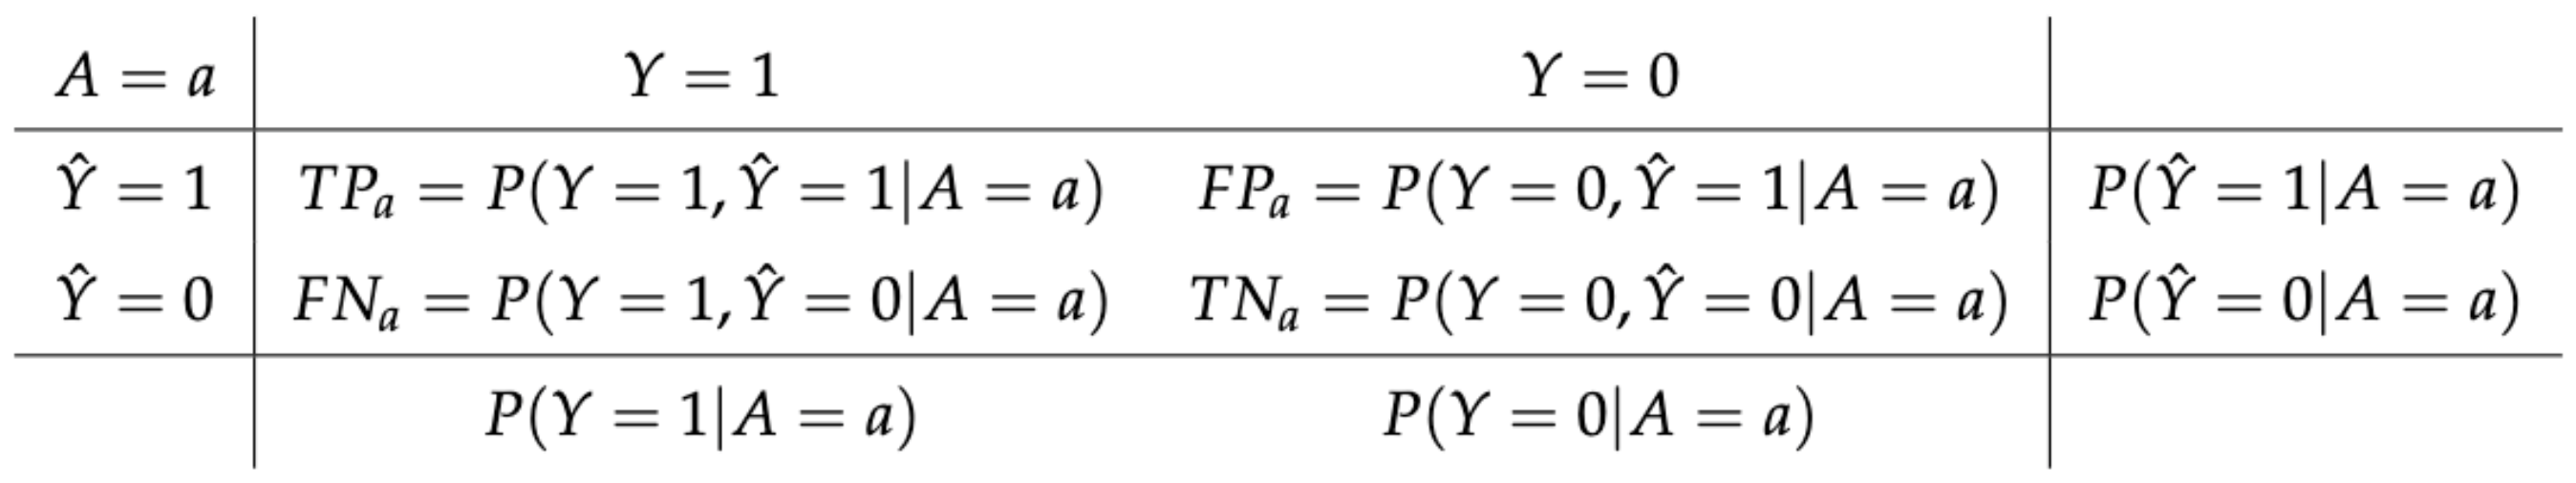
\includegraphics[width=1\linewidth]{table1} 

}

\caption[Summary of possible model outcomes for subpopulation $A = a$]{Summary of possible model outcomes for subpopulation $A = a$. We assume that outcome $Y = 1$ is favourable.}\label{fig:fairnessTable1}
\end{figure}
\end{Schunk}

According to \citet{barocas-hardt-narayanan} most discrimination
criteria can be derived as tests that validate the following
probabilistic definitions:

\begin{itemize}
\tightlist
\item
  Independence, i.e.~\(R \perp A\),
\item
  Separation, i.e.~\(R \perp A \mid Y\),
\item
  Sufficiency, i.e.~\(Y \perp A \mid R\).
\end{itemize}

Those criteria and their relaxations might be expressed via different
metrics based on a confusion matrix for a certain subgroup. To check if
those fairness criteria are addressed, we propose checking five metrics
among privileged group (a) and unprivileged group (b):

\begin{itemize}
\tightlist
\item
  Statistical parity:
  \(P(\hat{Y} = 1 | A = a) = P(\hat{Y} = 1 | A = b)\). Statistical
  parity (STP) ensures that fractions of assigned positive labels are
  the same in subgroups. It is equivalent of Independence
  \citep{statisticalparity}. In other words, the values in the last
  column of Figure \ref{fig:fairnessTable1} are the same for each
  subgroup.
\item
  Equal opportunity:
  \(P(\hat{Y} = 1 | A = a, Y = 1) = P(\hat{Y} = 1 | A = b, Y = 1)\).
  Checks if classifier has equal True Positive Rate (TPR) for each
  subgroup. In other words, the column normalized values in the second
  column of Figure \ref{fig:fairnessTable1} are the same for each
  subgroup. It is a relaxation of Separation \citep{NIPS20166374}.
\item
  Predictive parity:
  \(P(Y = 1 | A = a, \hat{Y} = 1) = P(Y = 1 | A = b, \hat{Y} = 1)\).
  Measures if a model has equal Positive Predictive Value (PPV) for each
  subgroup. In other words, the row normalized values in the second row
  of Figure \ref{fig:fairnessTable1} are the same for each subgroup. It
  is relaxation of Sufficiency \citep{ppv}.
\item
  Predictive equality:
  \(P(\hat{Y} = 1 | A = a, Y = 0) = P(\hat{Y} = 1 | A = b, Y = 0)\).
  Warrants that classifiers have equal False Positive Rate (FPR) for
  each subgroup. In other words, the column normalized values in the
  third column of Figure \ref{fig:fairnessTable1} are the same for each
  subgroup. It is relaxation of Separation \citep{ppe}.
\item
  (Overall) Accuracy equality:
  \(P(\hat{Y} = Y | A = a) = P(\hat{Y} = Y | A = b)\). Makes sure that
  models have the same Accuracy (ACC) for each subgroup.
  \citep{accuracy}
\end{itemize}

The reader should note that if the classifier passes Equal opportunity
and Predictive equality, it also passes Equalized Odds
\citep{NIPS20166374}, which is equivalent to Separation criteria.

Let us illustrate the intuition behind Independence, Separation, and
Sufficiency criteria using the well-known example of the COMPAS model
for estimating recidivism risk. Fulfilling the Independence criterion
means that the rate of sentenced prisoners should be equal in each
subpopulation. It can be said that such an approach is fair from
society's perspective.

Fulfilling the Separation criterion means that the fraction of
innocents/guilty sentenced should be equal in subgroups. Such an
approach is fair from the prisoner's perspective. The reasoning is the
following: \emph{``If I am innocent, I should have the same chance of
acquittal regardless of sub-population''}. This was the expectation
presented by the ProPublica Foundation in their study.

Meeting the Sufficiency criterion means that there should be an equal
fraction of innocents among the convicted, similarly, for the
non-convicted. This approach is fair from the judge's perspective. The
reasoning is the following: \emph{``If I convicted someone, he should
have the same chance of being innocent regardless of the
sub-population''}. This approach is presented by the company developing
the COMPAS model, Northpointe. Unfortunately, as we have already
written, it is not possible to meet all these criteria at the same time.

While defining the metrics above, we assumed only two subgroups. This
was done to facilitate notation, but there might be more unprivileged
subgroups. A perfectly fair model would pass all criteria for each
subgroup \citep{barocas-hardt-narayanan}.

Not all fairness metrics are equally important in all cases. The metrics
above aim to give a more holistic view into the fairness of the machine
learning model. Practitioners informed in the domain may consider only
those metrics that are relevant and beneficial from their point of view.
For example, in \citet{KOZODOI2021} in the fair credit scoring use case,
the authors concluded that the separation is the most suitable
non-discrimination criteria. More general instructions can also be found
in \citet{EUhandbook}, along with examples of protected attributes.
Sometimes, however, non-technical solutions to fairness problems might
be beneficial. Note that group fairness metrics will discover not all
types of unfairness, and the end-user should decide whether a model is
acceptable in terms of bias or not.

However tempting it is to think that all the criteria described above
can be met at the same time, unfortunately, this is not possible.
\citet{barocas-hardt-narayanan} shows that, apart from a few
hypothetical situations, no two of \emph{\{Independence, Separation,
Sufficiency\}} can be fulfilled simultaneously. So we are left balancing
between the degree of imbalance of the different criteria or deciding to
control only one criterion.

\hypertarget{bias}{%
\subsection{Acceptable amount of bias}\label{bias}}

It would be hard for any classifier to maintain the same relations
between subgroups. That is why some margins around the perfect agreement
are needed. To address this issue, we accepted the four-fifths rule
\citep{adverseimpact} as the benchmark for discrimination rate, which
states that \emph{``A selection rate for any race, sex, or ethnic group
which is less than four-fifths (\emph{\(\frac{4}{5}\)}) (or eighty
percent) of the rate for the group with the highest rate will generally
be regarded by the Federal enforcement agencies as evidence of adverse
impact{[}\ldots{]}.''} The selection rate is originally represented by
statistical parity, but we adopted this rule to define acceptable rates
between subgroups for all metrics. There are a few caveats to the
preceding citation concerning the size of the sample and the boundary
itself. Nevertheless, the four-fifths rule is an excellent guideline to
adhere to. In the implementation, this boundary is represented by
\(\varepsilon\), and it is adjustable by the user, but the default value
will be 0.8. This rule is often used, but users should check if the
fairness criteria should be set differently in each case.

Let \(\varepsilon > 0\) be the acceptable amount of a bias. In this
article, we would say that the model is not discriminatory for a
particular metric if the ratio between every unprivileged \(b, c, ...\)
and privileged subgroup \(a\) is within
\((\varepsilon, \frac{1}{\varepsilon})\). The common choice for the
epsilon is 0.8, which corresponds to the four-fifths rule. For example,
for the metric Statistical Parity (\(STP\)), a model would be
\(\varepsilon\)-non-discriminatory for privileged subgroup \(a\) if it
satisfies.

\begin{equation} 
\forall_{b \in A \setminus \{a\}} \;\;
   \varepsilon < STP_{ratio} = \frac{STP_b}{STP_a} < \frac{1}{\varepsilon}.
  \label{eq:ratio}
\end{equation}

\hypertarget{evaluating-fairness}{%
\subsection{Evaluating fairness}\label{evaluating-fairness}}

The main function in the \pkg{fairmodels} package is
\texttt{fairness\_check}. It returns \texttt{fairness\_object}, which
can be visualized or processed by other functions. This will be further
explained in the ``Structure'' section. When calling
\texttt{fairness\_check} for the first time, the following three
arguments are mandatory:

\begin{itemize}
\tightlist
\item
  \texttt{explainer} - an object that combines model and data that gives
  a unified interface for predictions. It is a wrapper over a model
  created with the \CRANpkg{DALEX} \citep{JMLRv19} package.
\item
  \texttt{protected} - a factor, vector containing sensitive attributes
  (protected group). It does not need to be binary. Instead, each level
  denotes a distinct subgroup. The most common examples are gender,
  race, nationality, etc.
\item
  \texttt{privileged} - a character/factor denoting a level in the
  protected vector which is suspected to be the most privileged one.
\end{itemize}

\hypertarget{example}{%
\subsubsection{Example}\label{example}}

In the following example, we are using \emph{German Credit Data} dataset
\citep{Dua2019}. In the dataset, there is information about people like
age, sex, purpose, credit amount, etc. For each person, there is a risk
assessed with taking credit, either good or bad. Therefore, it will be a
target variable. We will train the model on the whole dataset and then
measure fairness metrics to facilitate the notation (as opposed to
training and testing on different subsets, which is also possible and
advisable).

First, we create a model. Let's start with logistic regression.

\begin{Schunk}
\begin{Sinput}
library("fairmodels")
data("german")

lm_model <- glm(Risk~., data = german, family = binomial(link = "logit"))
\end{Sinput}
\end{Schunk}

\begin{example}
library("fairmodels")
data("german")

lm_model <- glm(Risk~., data = german, family = binomial(link = "logit"))
\end{example}

Then, create a wrapper that unifies the model interface.

\begin{Schunk}
\begin{Sinput}
library("DALEX")

y_numeric <- as.numeric(german$Risk) -1
explainer_lm <- DALEX::explain(lm_model, data = german[,-1], y = y_numeric)
\end{Sinput}
\end{Schunk}

Now we are ready to calculate and plot the fairness checks. Resulting
plot is presented in Figure \ref{fig:fairness-plot-1}.

\begin{Schunk}
\begin{Sinput}
fobject <- fairness_check(explainer_lm,
                protected = german$Sex, privileged = "male",
                verbose = FALSE)
\end{Sinput}
\end{Schunk}

\begin{Schunk}
\begin{Sinput}
plot(fobject)
\end{Sinput}
\begin{figure}

{\centering 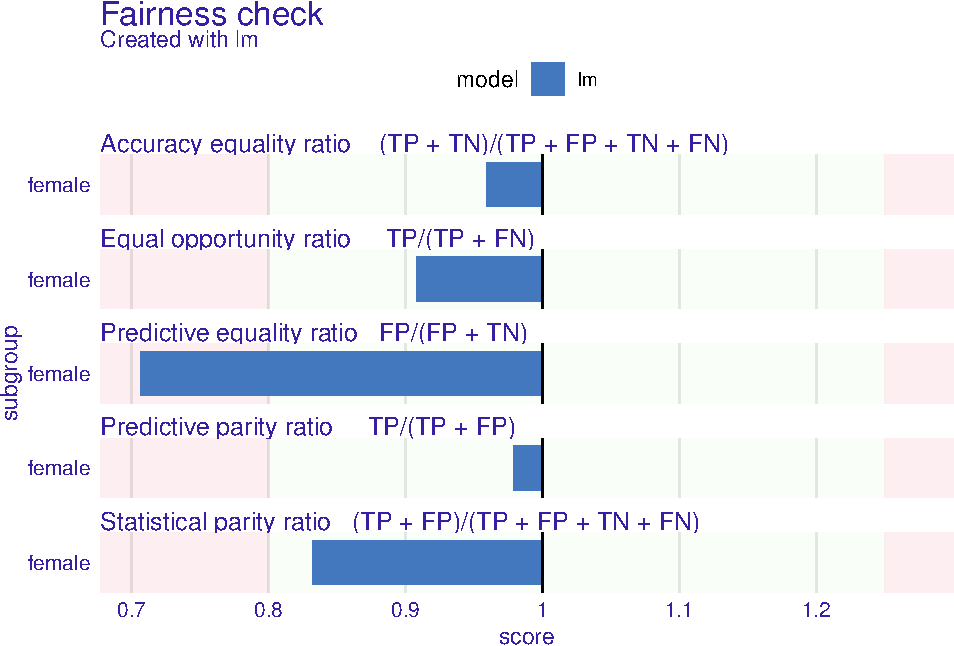
\includegraphics[width=0.75\linewidth]{RJ-2022-019_files/figure-latex/fairness-plot-1-1} 

}

\caption[The Fairness Check plot summarises the ratio of fairness measures between unprivileged and privileged subgroups]{The Fairness Check plot summarises the ratio of fairness measures between unprivileged and privileged subgroups. The light green areas correspond to values within $(\varepsilon, \frac{1}{\varepsilon})$ and signify an acceptable difference in fairness metrics. They are bounded by red rectangles indicating values that do not meet the 4/5 rule. Fairness metrics names are given along the formulas used to calculate the score in some subgroups to facilitate interpretation. For example, the ratio here means that after metric scores were calculated, the values for unprivileged groups (female) were divided by values for the privileged subgroup (male). In this example, except for the predictive equality ratio, the other measures are $\varepsilon$-non-discriminatory. }\label{fig:fairness-plot-1}
\end{figure}
\end{Schunk}

For a quick assessment, if a model passes fairness criteria, the object
created with \texttt{fairness\_check()} might be summarized with the
\texttt{print()} function. Total loss is the sum of all fairness
metrics. See equation \eqref{eq:parityLoss} for more details.

\begin{Schunk}
\begin{Sinput}
print(fobject, colorize = FALSE)
\end{Sinput}
\begin{Soutput}
#> 
#> Fairness check for models: lm 
#> 
#> lm passes 4/5 metrics
#> Total loss :  0.6153324
\end{Soutput}
\end{Schunk}

In this example, fairness criteria are satisfied in all but one metric.
The logistic regression model has a lower false-positive rate
(FP/(FP+TN))) in the unprivileged group than in the privileged group. It
exceeds the acceptable limit set by \(\varepsilon\). Thus it does not
satisfy the Predictive Equality ratio criteria.

More detailed visualizations are available, like \emph{Metric scores}
plot. It might be helpful to understand the intuition behind the
\emph{Fairness check} plot presented above. See an example in Figure
\ref{fig:fairness-plot-2}. This plot might be a good first point for
understanding the \emph{Fairness check} plot. In fact, checks can be
directly derived from the \emph{Metric scores} plot. To do this, we need
to divide the score denoted by the dot with the score denoted by the
vertical line. This way, we obtain a value indicated by the height of
the barplot. The orientation of the barplot depends on whether the value
is bigger or lower than 1. Intuitively the longer the horizontal line in
the figure below (the one connecting the dot with the vertical line) is,
the longer the bar will be in \emph{Fairness check} plot. If the scores
of privileged and unprivileged subgroups are the same, then the bar will
start from 1 and point to 1, so it will have a height equal to 0.

\begin{Schunk}
\begin{Sinput}
plot(metric_scores(fobject))
\end{Sinput}
\begin{figure}

{\centering 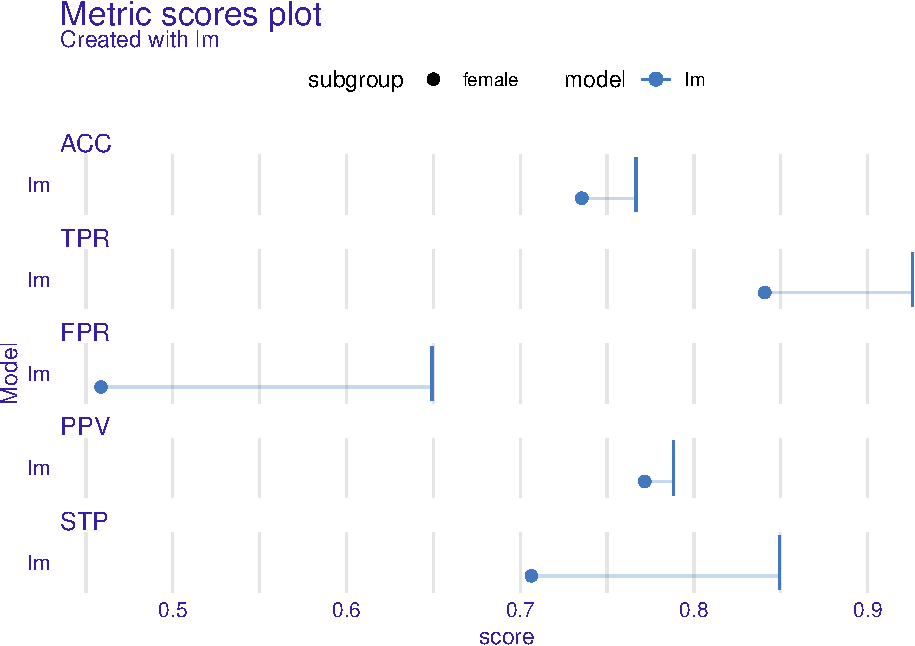
\includegraphics[width=0.75\linewidth]{RJ-2022-019_files/figure-latex/fairness-plot-2-1} 

}

\caption[The Metric Scores plot summarises raw fairness metrics scores for subgroups]{The Metric Scores plot summarises raw fairness metrics scores for subgroups. The dots stand for unprivileged subgroups (female) while vertical lines stans for the privileged subgroup (male). The horizontal lines act as a visual aid for measuring the difference between the scores of the metrics between the privileged and unprivileged subgroups.}\label{fig:fairness-plot-2}
\end{figure}
\end{Schunk}

It is rare that a model perfectly meets all the fairness criteria.
Therefore, a handy feature is the ability to compare several models on
the same scale. We add two more explainers to the fairness assessment in
the example below. Now \texttt{fairness\_object} (in code:
\texttt{fobject}) wraps three models together with different labels and
cutoffs for subgroups. The \texttt{fairness\_object} can be later used
as a basis for another \texttt{fairness\_object}. In detail, while
running \texttt{fairness\_check()} for the first time,
explainer/explainers have to be provided along with three arguments
described at the start of this section. However, as shown below, when
providing explainers with a \texttt{fairness\_object}, those arguments
are not necessary as they are already a part of the previously created
\texttt{fairness\_object}.

First, let us create two more models based on the \emph{German Credit
Data}. The first will be a logistic regression model that uses fewer
columns and has access to the \texttt{Sex} feature. The second is random
forest from \CRANpkg{ranger} \citep{ranger}. It will be trained on the
whole dataset.

\begin{Schunk}
\begin{Sinput}
discriminative_lm_model <- glm(Risk~.,
         data   = german[c("Risk", "Sex","Age",
                "Checking.account", "Credit.amount")],
         family = binomial(link = "logit"))

library("ranger")
rf_model <- ranger::ranger(Risk ~.,
         data = german, probability = TRUE,
         max.depth = 4, seed = 123)
\end{Sinput}
\end{Schunk}

These models differ in the way how the predict function works. To unify
operations on these models, we need to create \CRANpkg{DALEX} explainer
objects. The \texttt{label} argument specifies how these models are
named on plots.

\begin{Schunk}
\begin{Sinput}
explainer_dlm <- DALEX::explain(discriminative_lm_model,
        data = german[c("Sex", "Age", "Checking.account", "Credit.amount")],
        y = y_numeric,
        label = "discriminative_lm") 

explainer_rf <- DALEX::explain(rf_model, 
        data = german[,-1], y = y_numeric)
\end{Sinput}
\end{Schunk}

Now we are ready to assess fairness. The resulting plot is presented in
Figure \ref{fig:fairness-plot-3}.

\begin{Schunk}
\begin{Sinput}
fobject <- fairness_check(explainer_rf, explainer_dlm, fobject)
plot(fobject)
\end{Sinput}
\begin{figure}

{\centering 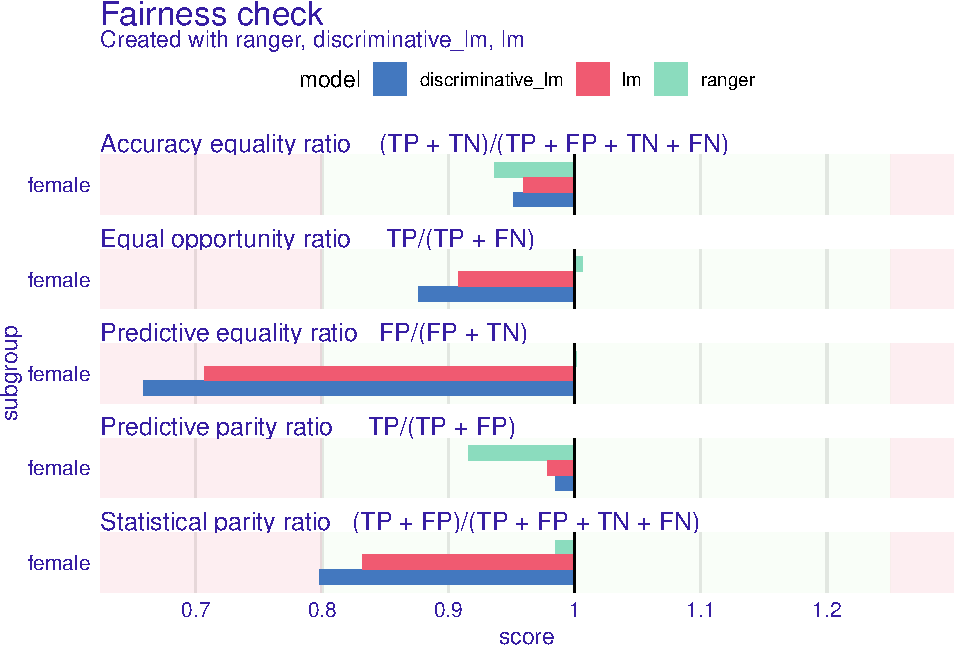
\includegraphics[width=0.75\linewidth]{RJ-2022-019_files/figure-latex/fairness-plot-3-1} 

}

\caption[The Fairness Check plot for multiple models]{The Fairness Check plot for multiple models. It helps to compare models based on five selected fairness measures. }\label{fig:fairness-plot-3}
\end{figure}
\end{Schunk}

When plotted, new bars appear on the fairness check plot. Those are new
metric scores for added models. This information can be summarized in a
numerical way with the \texttt{print()} function.

\begin{Schunk}
\begin{Sinput}
print(fobject, colorize = FALSE)
\end{Sinput}
\begin{Soutput}
#> 
#> Fairness check for models: ranger, discriminative_lm, lm 
#> 
#> ranger passes 5/5 metrics
#> Total loss :  0.1699186 
#> 
#> discriminative_lm passes 3/5 metrics
#> Total loss :  0.7294678 
#> 
#> lm passes 4/5 metrics
#> Total loss :  0.6153324
\end{Soutput}
\end{Schunk}

\hypertarget{package-architecture}{%
\section{Package architecture}\label{package-architecture}}

The \pkg{fairmodels} package provides a unified interface for predictive
models independently of their internal structure. Using a model agnostic
approach with \pkg{DALEX} explainers facilitates this process
\citep{JMLRv19}. There is a unified way for each explainer to check if
explained model lives up to user fairness standards. Checking fairness
with \pkg{fairmodels} is straightforward and can be done with the
three-step pipeline.

\begin{verbatim}
classification model   |>   explain()   |>   fairness_check() 
\end{verbatim}

The output of such a pipeline is an object of class
\texttt{fairness\_object}, a unified structure to wrap model explainer
or multiple model explainers and other \texttt{fairness\_objects} in a
single container. Aggregation of fairness measures is done based on
groups defined by model labels. This is why model explainers (even those
wrapped by \texttt{fairness\_objects}) must have different labels.
Moreover, some visualizations for model comparison assume that all
models are created from the same data. Of course, each model can use
different variables or different feature transformations, but the order
and number of rows shall stay the same. To facilitate aggregation of
models \pkg{fairmodels} allows creating \texttt{fairness\_objects} in
other ways:

\begin{itemize}
\tightlist
\item
  \texttt{explainers\ \textbar{}\textgreater{}\ fairness\_check()} -
  possibly many explainers can be passed to \texttt{fairness\_check()},
\item
  \texttt{fairness\_objects\ \textbar{}\textgreater{}\ fairness\_check()}
  - explainers stored in \texttt{fairness\_objects} passed to
  \texttt{fairness\_check()} will be aggregated into one
  \texttt{fairness\_object},
\item
  \texttt{explainer} \&
  \texttt{fairness\_objects\ \textbar{}\textgreater{}\ fairness\_check()}
  - explainers passed directly and explainers from
  \texttt{fairness\_objects} will be aggregated into one
  \texttt{fairness\_object}.
\end{itemize}

When using the last two pipelines, protected vectors and privileged
parameters are assumed to be the same, so passing them to
\texttt{fairness\_check()} is unnecessary.

To create a \texttt{fairness\_object}, at least one explainer needs to
be passed to \texttt{fairness\_check()} function, which returns the said
object. \texttt{fairness\_object} metrics for each subgroup are
calculated from the separate confusion matrices.

The \texttt{fairness\_object} has numerous fields. Some of them are:

\begin{itemize}
\tightlist
\item
  \texttt{parity\_loss\_metric\_data} - data.frame containing parity
  loss for each metric and classifier,
\item
  \texttt{groups\_data} - list of metric scores for each metric and
  model,
\item
  \texttt{group\_confusion\_matrices} - list of values in confusion
  matrices for each model and metric,
\item
  \texttt{explainers} - list of DALEX explainers. When explainers and/or
  \texttt{fairness\_object} are added, then explainers and/or explainers
  extracted from \texttt{fairness\_object} are added to that list,
\item
  \texttt{label} - character vector of labels for each explainer.
\item
  \texttt{...} - other fields.
\end{itemize}

The \texttt{fairness\_object} methods are used to create numerous
objects that help to visualize bias. In the next sections, we list more
detailed functions for deeper exploration of bias. Detailed relations
between objects created with \pkg{fairmodels} are depicted in Figure
\ref{fig:classdiagram}. The general overview of the workflow is
presented in Figure \ref{fig:flowchart}.

\begin{Schunk}
\begin{figure}

{\centering 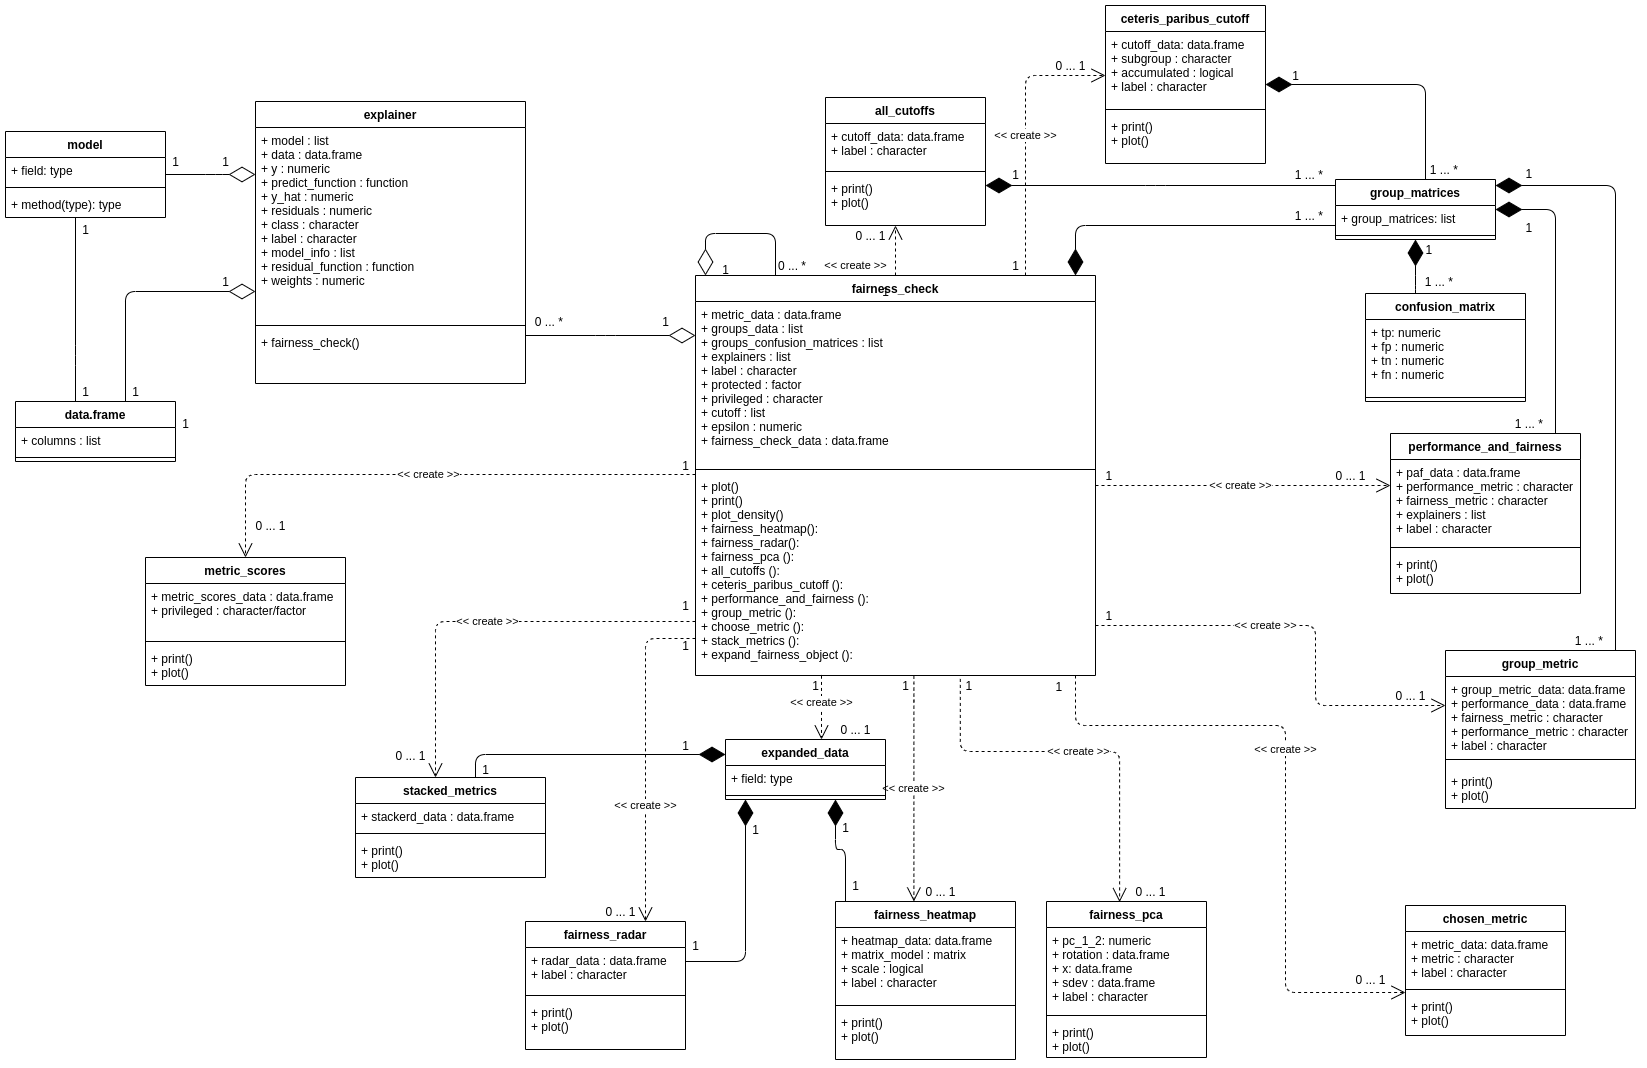
\includegraphics[width=1\linewidth]{class_diagram} 

}

\caption[Class diagram for objects created by functions from the fairmodels package]{Class diagram for objects created by functions from the fairmodels package. Each rectangle corresponds to one class, the name of this class is in the header of the rectangle. Each of these classes is a list containing a certain list of objects. The top slot lists the names and types of each object the list. The bottom slot contains a list of functions that can be performed on objects of the specified class. If two classes are connected by a line ending in a diamond it means that one class contains objects of the other class. If two rectangles are connected by a dashed line, it means that on the basis of one object, an object of another class can be produced. In this case, more detailed fairness statistics can be produced from the central object of the fairness check class. See the full resolution at https://bit.ly/3HNbNvo}\label{fig:classdiagram}
\end{figure}
\end{Schunk}

\begin{Schunk}
\begin{figure}

{\centering 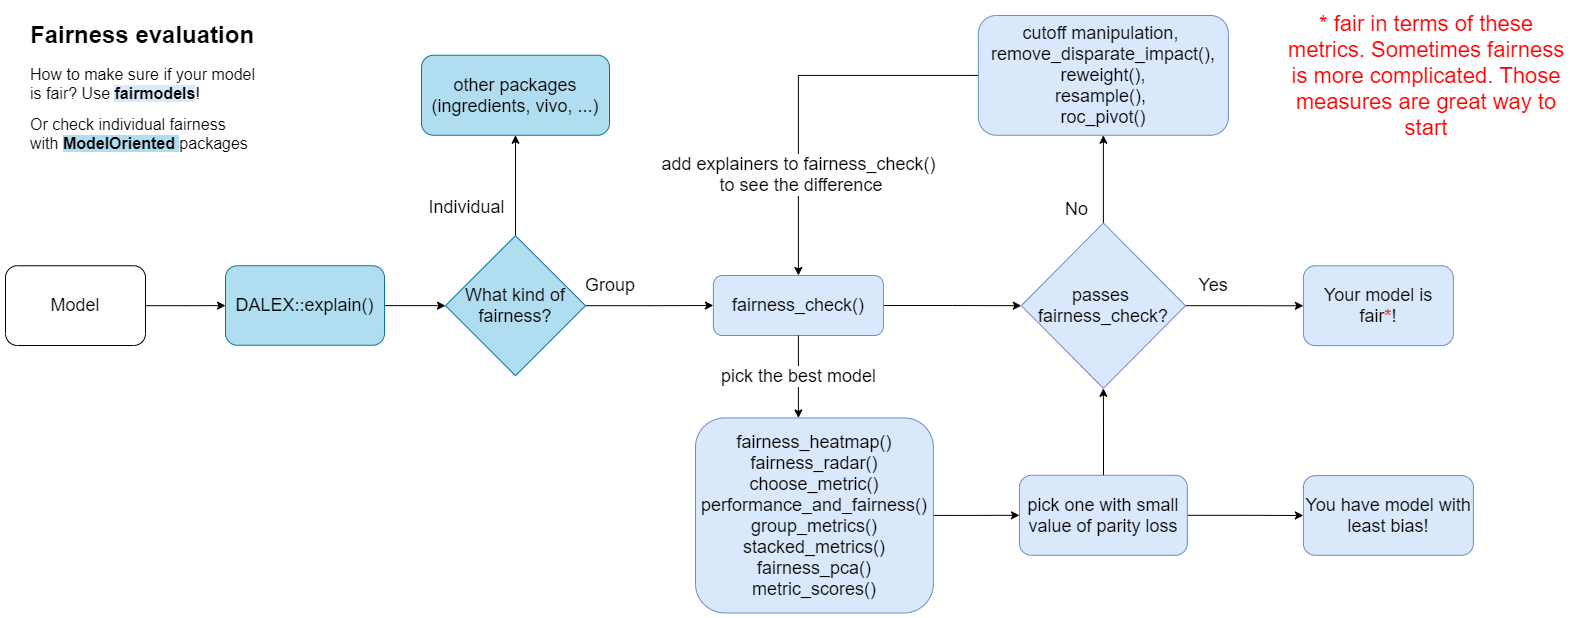
\includegraphics[width=1\linewidth]{flow} 

}

\caption[Flowchart for the fairness assessment with the fairmodels package]{Flowchart for the fairness assessment with the fairmodels package. The arrows describe typical sequences of actions when exploring the fairness of the models. For ease of use, the names of the functions that can be used in a given step are indicated. Note that this procedure is intended to look at the model from multiple perspectives in order to track down potential problems in the model. Merely satisfying the fairness criteria does not automatically mean that the model is free of any errors}\label{fig:flowchart}
\end{figure}
\end{Schunk}

\hypertarget{visualization}{%
\section{Visualizing bias}\label{visualization}}

In \pkg{fairmodels} there are 12 metrics based on confusion matrices for
each subgroup, see the following table for the complete list. Some of
them were already introduced before.

\begin{table}[h!]
\begin{center}
\footnotesize
    \begin{tabular}{p{1cm}p{2.6cm}p{3.8cm}p{4cm}}
    \hline
Metric & Formula & Name & Fairness criteria \\ \hline    
TPR & $\frac{TP}{TP + FN}$ & True positive rate & Equal opportunity \newline\citep{NIPS20166374} \\ \hline
TNR & $\frac{TN}{TN + FP}$ & True negative rate & \\ \hline
PPV & $\frac{TP}{TP + FP}$ & Positive predictive value & Predictive parity \newline\citep{ppv}\\ \hline
NPV & $\frac{TN}{TN + FN}$ & Negative predictive value & \\ \hline
FNR & $\frac{FN}{FN + TP}$ & False negative rate & \\ \hline
FPR & $\frac{FP}{FP + TN}$ & False positive rate & Predictive equality \newline\citep{ppe} \\ \hline
FDR & $\frac{FP}{FP + TP}$ & False discovery rate &\\ \hline
FOR & $\frac{FN}{FN + TN}$ & False omission rate & \\ \hline
TS & $\frac{TP}{TP + FN + FP}$  & Threat score &\\ \hline
STP & $\frac{TP + FP}{TP + FP + TN + FN}$ & Positive rate & Statistical parity \newline \citep{statisticalparity}\\ \hline
ACC & $\frac{TP + TN}{TP + TN + FP + FN}$ & Accuracy & Overall accuracy equality \newline\citep{accuracy} \\ \hline
F1 &  $\frac{2 \cdot PPV * TPR}{PPV + TPR}$ & F1 score &\\ \hline
    \end{tabular}
    \caption{Fairness metrics implemented in the \textbf{fairmodels} package}
\label{tab:Metrics-table}
\end{center}
\end{table}

Not all metrics are needed to determine if the discrimination exists,
but they are helpful to acquire a fuller picture. To facilitate the
visualization over many subgroups, we introduce a function that maps
metric scores among subgroups to a single value. This function, which we
call \texttt{parity\_loss}, has an attractive property. Due to the usage
of the absolute value of the natural logarithm, it will return the same
value whether the ratio is inverted or not.

So, for example, when we would like to know the parity loss of
Statistical Parity between unprivileged (b) and privileged (a)
subgroups, we mean value like this:

\begin{equation} 
STP_{\textit{parity loss}} = \Big | \ln \Big( \frac{STP_b}{STP_a} \Big)\Big|. 
\end{equation}

This notation is very helpful because it allows to accumulate
\(STP_{\textit{parity loss}}\) overall unprivileged subgroups, so not
only in the binary case.

\begin{equation} 
STP_{\textit{parity loss}} = \sum_{i \in \{a, b, ...\}} \Big|\ln \Big(\frac{STP_i}{STP_a} \Big)\Big|.  
  \label{eq:parityLoss}
\end{equation}

The \texttt{parity\_loss} relates strictly to ratios. The classifier is
more fair if \texttt{parity\_loss} is low. This property is helpful in
visualizations.

There are several modifying functions that operate on
\texttt{fairness\_object}. Their usage will return other objects. The
relations between them is depicted on the class diagram (Figure
\ref{fig:classdiagram}). The objects can then be plotted with a generic
\texttt{plot()} function. Additionally, a special plotting function
works immediately on \texttt{fairness\_object}, which is
\texttt{plot\_density}. The user can directly specify which metrics
shall be visible in the plot in some functions. The detailed technical
introduction for all these functions is presented in
\href{https://cran.r-project.org/web/packages/fairmodels/fairmodels.pdf}{\pkg{fairmodels} manual}.

\clearpage

Plots visualizing different aspects of \texttt{parity\_loss} can be
created with one of the following pipelines:

\begin{itemize}
\tightlist
\item
  \texttt{fairness\_object\ \textbar{}\textgreater{}\ modifying\_function(...)\ \textbar{}\textgreater{}\ plot()}\strut \\
  This pipe is preferred and allows setting parameters in both modifying
  functions and certain plot functions, which is not the case with the
  next pipeline.
\item
  \texttt{fairness\_object\ \textbar{}\textgreater{}\ plot\_fairmodels(type\ =\ modifying\_function,\ ...)}\strut \\
  Additional parameters are passed to the modifying functions and not to
  the plot function.
\end{itemize}

Using the pipelines, different plots can be obtained by superseding the
\texttt{modifying\_function} with function names. Four examples of
additional graphical functions available in the \texttt{fairmodels} can
be seen in Figure \ref{fig:all}. This package implements a total of 8
different diagnostic plots, each describing a different fairness
perspective. To see different aspects of fairness and bias, the user can
choose the model with the smallest bias, find out the similarity between
metrics and models, compare models in both fairness and performance, and
see how cutoff manipulation might change the \texttt{parity\_loss}. Find
more information about each of them in the documentation.

\begin{Schunk}
\begin{Sinput}
fp1  <- plot(ceteris_paribus_cutoff(fobject, "male", cumulated=TRUE))
fp2  <- plot(fairness_heatmap(fobject))
fp3  <- plot(stack_metrics(fobject))
fp4  <- plot(plot_density(fobject))
\end{Sinput}
\end{Schunk}

\begin{Schunk}
\begin{Sinput}
library("patchwork")
fp1 + fp2 + fp3 + fp4 + 
  plot_layout(ncol = 2)
\end{Sinput}
\begin{figure}

{\centering 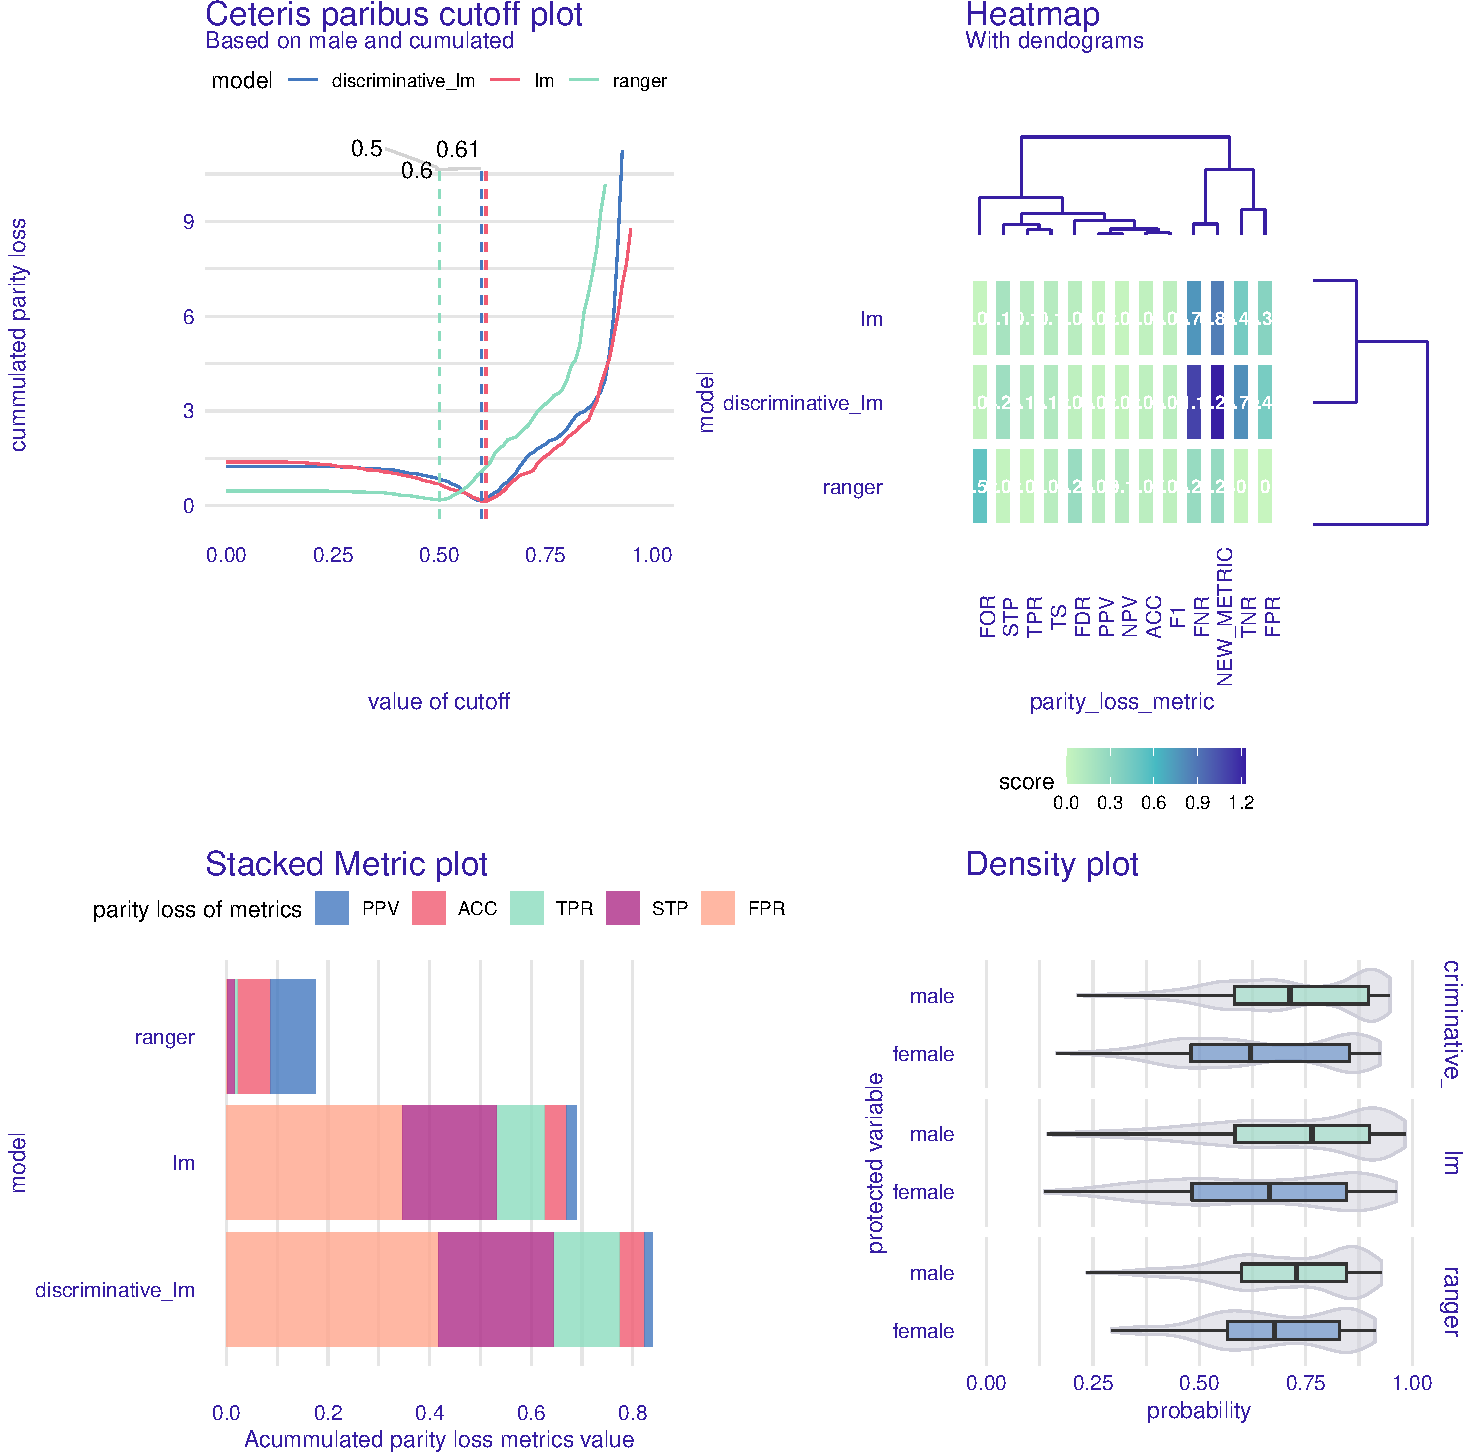
\includegraphics[width=1\linewidth]{RJ-2022-019_files/figure-latex/all-1} 

}

\caption[Four examples of additional graphical functions are available in the fairmodels package that facilitates model and bias exploration]{Four examples of additional graphical functions are available in the fairmodels package that facilitates model and bias exploration. The Ceteris Paribus Cuttoff plot helps select the cutoff values for each model to maximize a particular measure of fairness. In this case, the suggested cutoff point for both linear models is similar. However, the ranger model does not have calibrated probabilities and thus requires a different cutoff. The Heatmap plot is very helpful when comparing large numbers of models. It shows profiles of selected fairness measures for each of the models under consideration. In this case, the fairness profiles for both linear models are similar. The Stacked Metric plot helps you compare models by summing five different fairness measures. The different layers of this plot allow you to compare individual measures, but if you don't know which one to focus on, it is useful to look at the sum of the measures. In this case, the ranger model has the highest fairness values. Finally, the Density plot helps to compare the score distributions of the models between the advantaged and disadvantaged groups. In this case, we find that for females the distributions of the scores are lower in all models, with the largest difference for the lm model. }\label{fig:all}
\end{figure}
\end{Schunk}

\hypertarget{mitigation}{%
\section{Bias mitigation}\label{mitigation}}

What can be done if the model does not meet the fairness criteria?
Machine learning practitioners might use other algorithms or variables
to construct unbiased models, but this does not guarantee passing the
\texttt{fairness\_check()}. An alternative is to use bias mitigation
techniques that adjust the data or model to meet fairness conditions.
There are essentially three types of such methods. The first is data
pre-processing. There are many ways to ``correct'' the data when there
are unwanted correlations between variables or sample sizes among
subgroups in data. The second one is in-processing, which is, for
example, optimizing classifiers not only to reduce classification error
but also to minimize a fairness metric. Last but not least is
post-processing which modifies model output so that predictions and
miss-predictions among subgroups are more alike.

The \pkg{fairmodels} package offers five functions for bias mitigation,
three for pre-processing, and two for post-processing. Most of these
approaches are also implemented in
\href{https://aif360.mybluemix.net/}{aif360} \citep{aif360-oct-2018}.
However, in \pkg{fairmodels} there are separate implementations of them
in R. There are a lot of useful mitigation techniques that are not in
\pkg{fairmodels} like those in \citet{NIPS20166374} and numerous
in-processing algorithms.

\hypertarget{data-pre-processing}{%
\subsection{Data pre-processing}\label{data-pre-processing}}

\begin{itemize}
\tightlist
\item
  \textbf{Disparate impact remover}\\
  In \pkg{fairmodels} geometric repair, an algorithm originally
  introduced by \citet{disparateImpact}, works on ordinal, numeric
  features. Depending on the \(\lambda \in [0,1]\) parameter, this
  method will transform the distribution of a given feature. The idea is
  simple. Given feature distribution in different subgroups, the
  algorithm finds optimal distribution (according to earth mover's
  distance) and transforms distribution for each subgroup to match the
  optimal one. For example, if age is an important feature and its
  distribution is different in two subgroups, and we want to change
  that, then the geometric repair will map each individual's age to a
  new distribution (different age). It will be preserving the order -
  the ranks (in our case, seniority) of observations are preserved.
  Parameter \(\lambda\) is responsible for the repair degree, so for
  full repair, lambda should be set to 1. The method does not focus on a
  particular metric but rather tries to level out them by transforming
  potentially harmful feature distributions.
\item
  \textbf{Reweighting}\\
  Reweighting is a rather straightforward approach. This method was
  implemented according to \citet{kamiran}. It computes weights by
  dividing the theoretical probability of assigning favorable labels for
  a subgroup by real (observed) probability (based on the data).
  Theoretic probability for a subgroup is computed by multiplying the
  probability of assigning a favorable label (for all populations) by
  picking observation from a certain subgroup. It focuses on mitigating
  statistical parity.
\item
  \textbf{Resampling}\\
  Resampling is based on weights calculated in \texttt{reweighting}.
  Each weight for a subgroup is multiplied by the size of the subgroup.
  Then, whether the subgroup is deprived or not (if weight is higher
  than one, the subgroup is considered deprived), observations are
  duplicated from either one that were assigned a favorable label or
  not. There are two types of resampling- uniform and preferential. The
  uniform is making algorithm pick or omit observations randomly without
  considering its probabilistic score. Preferential uses another
  probabilistic classifier, potentially different from the main model
  for final predictions. In \citet{kamiran} it is called ranker - it
  predicts the probabilities for the observations to decide which
  observations are close to the cutoff border (usually 0.5). Based on
  the probabilistic output of the ranker, the observations are sorted,
  and the ones with the highest/lowest ranks are either left out or
  duplicated depending on the case---more on that on \citet{kamiran}.
  The \pkg{fairmodels} implementation, instead of training the ranker as
  in the aforementioned paper, uses a vector of previously calculated
  probabilities provided by the user. With this, it shifts the decision
  and responsibility of choosing a ranker to the user. It focuses on
  mitigating statistical parity.
\end{itemize}

\hypertarget{model-post-processing}{%
\subsection{Model post-processing}\label{model-post-processing}}

\begin{itemize}
\tightlist
\item
  \textbf{Reject Option based Classification Pivot}\\
  The \texttt{roc\_pivot} method is implemented based on
  \citet{postKamiran} in the \pkg{fairmodels} package. Let
  \(\theta \in (0,1)\) be the value that determines the radius of the
  so-called critical region, which is an area around the cutoff. The
  user specifies the \(\theta\), and it should describe how big the
  critical region should be. For example if \(\theta = 0.1\) and cutoff
  is 0.6, then the critical region will be (0.5, 0.7). Let's assume that
  we are predicting a favorable outcome. If the assigned probability of
  observation is in the described region, then the probabilities are
  pivoting on the other side of the cutoff with a certain assumption. If
  an observation in a critical region is considered to be the privileged
  and it is on the right side of the cutoff, then its probabilities are
  pivoting from the right side of the cutoff to the left. So if an
  observation is in the critical region and it is considered
  unprivileged, then if it is on the left side of the cutoff, it will
  pivot to the right side. Pivoting here means changing the side of the
  cutoff so that the distance from the cutoff stays unchanged. It does
  not intend to mitigate a single metric but rather changes predictions
  in the critical region (the region with low certainty). By pivoting
  the predictions, it might lower more metrics.\\
\item
  \textbf{Cutoff manipulation}\\
  The \pkg{fairmodels} package supports setting cutoff for each
  subgroup. Users may pick \texttt{parity\_loss} metrics of their choice
  and find the minimal \texttt{parity\_loss}. It is part of
  \texttt{ceteris\_paribus\_cutoff()} function. Based on picked metrics,
  the sum of parity loss is calculated for each cutoff of the chosen
  subgroup. Then the minimal value is found---this way, optimal values
  might be found for metrics of interest. The minimum is marked with a
  dashed vertical line (see Figure \ref{fig:all}). This approach however
  might be to some extent concerning. Some might argue that setting
  different cutoffs for different subgroups is unfair and is punishing
  privileged subgroups for something they have no control of. Especially
  in the individual fairness field, it would be concerning if two
  similar people with different sensitive attributes would have two
  different thresholds and potentially two different outcomes. This is a
  valid point, and this method should be used with knowledge of all its
  drawbacks. The cutoff manipulation method targets metrics chosen by
  the user.
\end{itemize}

All pre-processing methods can be used with two pipelines, whereas
post-processing can be used in one specific way.

\begin{itemize}
\tightlist
\item
  Pre-processing pipelines

  \begin{itemize}
  \tightlist
  \item
    \texttt{data/explainer\ \textbar{}\textgreater{}\ method}\strut \\
    Returns either weights, indexes, or changed data depending on the
    method used.
  \item
    \texttt{data/explainer\ \textbar{}\textgreater{}\ pre\_process\_data(data,\ protected,\ y,\ type\ =\ ...)}\strut \\
    Always returns data.frame. In case of weights data has additional
    column called \texttt{\_weights\_}.
  \end{itemize}
\item
  Post-processing pipelines

  \begin{itemize}
  \tightlist
  \item
    \texttt{fairness\_object\ \textbar{}\textgreater{}\ ceteris\_paribus\_cutoff(subgroup,\ ...)\ \textbar{}\textgreater{}\ print/plot}\strut \\
    This is the pipeline for creating ceteris paribus cutoff print and
    plot.
  \item
    \texttt{explainer\ \textbar{}\textgreater{}\ roc\_pivot(protected,\ privileged,\ ...)}\strut \\
    The pipeline will return explainer with \texttt{y\_hat} field
    changed.
  \end{itemize}
\end{itemize}

The user should be aware that debiasing one metric might enhance bias in
another. It is a so-called fairness-fairness trade-off. There is also a
fairness-performance trade-off where debiasing one metric leads to worse
performance. Another thing to remember is, as found in
\citet{Agrawal2020DebiasingCI}, metrics might not generalize well to
out-of-distribution examples, so it is advised also to check the
fairness metrics on a separate test set.

\hypertarget{example-1}{%
\subsection{Example}\label{example-1}}

Now we will show an example usage of one pre-processing and one
post-processing method. As before, the \textbf{German Credit Data} will
be used along with the previously created \texttt{lm\_model}. So
firstly, we create a new dataset using \texttt{pre\_process\_data} and
then we use it to train the logistic regression classifier.

\begin{Schunk}
\begin{Sinput}
resampled_german   <- german |> pre_process_data(protected = german$Sex,
                y_numeric, type = 'resample_uniform')

lm_model_resample  <- glm(Risk~.,
                data   = resampled_german,
                family = binomial(link = "logit"))

explainer_lm_resample <- DALEX::explain(lm_model_resample,
                data = german[,-1], y = y_numeric, verbose = FALSE)
\end{Sinput}
\end{Schunk}

Then we make other explainers. We use previously created
\texttt{explainer\_lm} with the post-processing function
\texttt{roc\_pivot}. We set parameter \texttt{theta\ =\ 0.05} for a
rather narrow area of a pivot.

\begin{Schunk}
\begin{Sinput}
new_explainer <- explainer_lm |> roc_pivot(protected = german$Sex,
                privileged = "male", theta = 0.05)
\end{Sinput}
\end{Schunk}

In the end, we create \texttt{fairness\_object} with explainers obtained
with the code above and one created in the first example to see the
difference.

\begin{Schunk}
\begin{Sinput}
fobject <- fairness_check(explainer_lm_resample, new_explainer, explainer_lm,
                protected = german$Sex, privileged = "male",
                label = c("resample", "roc", "base"),
                verbose = FALSE)

fobject |> plot()
\end{Sinput}
\begin{figure}

{\centering 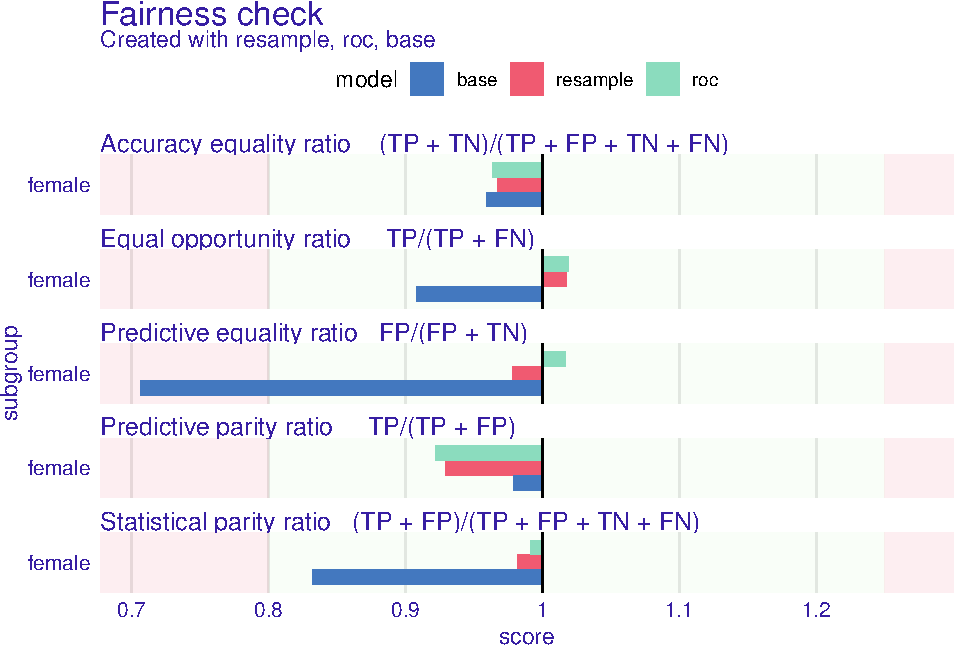
\includegraphics[width=0.8\linewidth]{RJ-2022-019_files/figure-latex/mitigation-1} 

}

\caption[Graphical summary of a base model (blue bars) and model after applying two bias mitigation techniques (red and green bars)]{Graphical summary of a base model (blue bars) and model after applying two bias mitigation techniques (red and green bars). By comparing adjacent rectangles one can read how the respective technique affected the corresponding fairness measure}\label{fig:mitigation}
\end{figure}
\end{Schunk}

The result of the code above is presented in Figure
\ref{fig:mitigation}. The mitigation methods successfully eliminated
bias in all of the metrics. Both models are better than the original
\texttt{base}. This is not always the case - sometimes, eliminating bias
in one metric may increase bias in another metric. For example, let's
consider a perfectly accurate model, but some subgroups receive few
positive predictions (bias in Statistical parity). In that case,
mitigating the bias in Statistical parity would decrease the Accuracy
equality ratio.

\hypertarget{summary-and-future-work}{%
\section{Summary and future work}\label{summary-and-future-work}}

This paper showed that checking for bias in machine learning models can
be done conveniently and flexibly. The package \pkg{fairmodels}
described above is a self-sufficient tool for bias detection,
visualization, and mitigation in classification machine learning models.
We presented theory, package architecture, suggested usage, and examples
along with plots. Along the way, we introduced the core concepts and
assumptions that come along the bias detection and plot interpretation.
The package is still improved and enhanced, which can be seen by adding
the announced regression module based on \citet{regression}. We did not
cover it in this article because it is still an experimental tool.
Another tool for in-processing classification closely related to
\pkg{fairmodels} has also been added and can be found on
\url{https://github.com/ModelOriented/FairPAN}.

The source code of the package, vignettes, examples, and documentation
can be found at \url{https://modeloriented.github.io/fairmodels/}. The
stable version is available on CRAN. The code and the development
version can be found on GitHub
\url{https://github.com/ModelOriented/fairmodels}. This is also a place
to report bugs or requests (through GitHub issues).

In the future, we plan to enhance the spectrum of bias visualization
plots and introduce regression and individual fairness methods. The
potential way to explore would be an in-processing bias mitigation -
training models that minimize cost function and adhere to certain
fairness criteria. This field is heavily developed in Python and lacks
appropriate attention in R.

\hypertarget{acknowledgements}{%
\section*{Acknowledgements}\label{acknowledgements}}
\addcontentsline{toc}{section}{Acknowledgements}

Work on this package was financially supported by the NCN Sonata Bis-9
grant 2019/34/E/ST6/00052.

\bibliography{Wisniewski-Biecek.bib}

\address{%
Jakub Wiśniewski\\
Warsaw University of Technology\\%
Faculty of Mathematics and Information Science\\ Poland\\
%
%
%
\href{mailto:jakwisn@gmail.com}{\nolinkurl{jakwisn@gmail.com}}%
}

\address{%
Przemysław Biecek\\
Warsaw University of Technology\\%
Faculty of Mathematics and Information Science\\ University of
Warsaw\\ Faculty of Mathematics, Informatics, and Mechanics\\ Poland\\
%
\url{https://pbiecek.github.io/}\\%
\textit{ORCiD: \href{https://orcid.org/0000-0001-8423-1823}{0000-0001-8423-1823}}\\%
\href{mailto:przemyslaw.biecek@pw.edu.pl}{\nolinkurl{przemyslaw.biecek@pw.edu.pl}}%
}
